\section{SWIRL: Learning With Transition States}
\label{swirl}
Next, we build on TSC to construct a planner that leverages the structure learned by TSC.
Real-world tasks often naturally decompose into a sequence of simpler, locally-solvable sub-tasks.
For example, an assembly task might decompose into completing the part's constituent sub-assemblies or a surgical task might decompose into a sequence of movement primitives.
Such structure imposes a strong prior on the class of successful policies and can focus exploration in reinforcement learning.
It reduces the effective time horizon of learning to the start of the next subtask rather than until task completion.
We apply a clustering algorithm to identify a latent set of state-space subgoals that sequentially compose to form the global task.
This leads to a novel policy search algorithm, called Sequential Windowed Inverse Reinforcement Learning (SWIRL),  where the demonstrations can bootstrap a self-supervised Q-learning algorithm.

 Transitions are defined as significant changes in the state trajectory. These transitions can be spatially and temporally clustered to identify if there are common conditions that trigger a change in motion across demonstrations.
SWIRL extends this basic model with an Inverse Reinforcement Learning step that extracts subgoals and computes local cost functions from the learned clusters. 
Learning a policy over the segmented task is nontrivial because solving $k$ independent problems neglects any shared structure in the value function during the policy learning phase (e.g., a common failure state).
Jointly learning over all segments introduces a dependence on history, namely, any policy must complete step $i$ before step $i+1$.
Learning a memory-dependent policy could lead to an exponential overhead of additional states. 
We show that the problem can be posed as a proper MDP in a lifted state-space that includes an indicator variable of the highest-index $\{1,...,k\}$ transition region that has been reached so far if there are Markovian regularity assumptions on the clustering algorithm.

\subsection*{Model and Notation}
Directly optimizing the reward function $\mathcal{R}$ in the MDP from the previous section might be very challenging.
We propose to approximate $\mathcal{R}$ with a sequence of smoother reward functions.

\begin{definition}[Proxy Task]
A proxy task is a set of $k$ MDPs with the same state set, action set, and dynamics. 
Associated with each MDP $i$ is a reward function  $R_i: S \times A \mapsto \mathbb{R}$. Additionally, associated with each $R_i$ is a transition region $\rho_i \subseteq S$, which is a subset of the state-space. A robot accumulates a reward $R_i$ until it reaches the transition $\rho_i$, then the robot switches to the next reward and transition pair.
This process continues until $\rho_k$ is reached.
\end{definition}

A robot is deemed \emph{successful} when all of the $\rho_i$ are reached in sequence within a global time-horizon $T$. \hirl uses a set of initial supervisor demonstrations to construct a proxy task that approximates the original MDP. To make this problem computationally tractable, we make some modeling assumptions.

\vspace{0.5em}\noindent\textbf{Modeling Assumption 1. Successful Demonstrations: } We need conditions on the demonstrations to be able to infer the sequential structure. We assume that all demonstrations are successful, that is, they visit each $\rho_i$ in the same sequence.

\vspace{0.5em}\noindent\textbf{Modeling Assumption 2. Quadratic Rewards: } We assume that each reward function $R_i$ can be expressed as a quadratic of the form $-(s-s_0)^T \Psi (s - s_0)$ for some positive semi-definite $\Psi$ and a center point $s_0$ with $s_0^T \Psi s_0 = 0$. 

\vspace{0.5em}\noindent\textbf{Modeling Assumption 3. Ellipsoidal Approximation: } Finally, we assume that the transition regions in $\rho_i$ can be approximated by a set of disjoint ellipsoids.

\subsubsection{Algorithm Overview}
\hirl can be described in terms of three sub-algorithms:

\vspace{4pt}

\noindent\textbf{Inputs:} Demonstrations $D$
\begin{enumerate}
    \item \textbf{Sequence Learning: } Given $D$, \hirl applies \tsc to partition the task into $k$ sub-tasks whose start and end are defined by arrival at a sequence of transitions $G = [\rho_1,...,\rho_k]$.
    \item \textbf{Reward Learning: } Given $G$ and $D$, \hirl associates a local reward function with each segment resulting in a sequence of rewards $\mathbf{R}_{seq} = [R_1,...,R_k]$. 
    \item \textbf{Policy Learning: } Given $\mathbf{R}_{seq}$ and $G$, \hirl applies reinforcement learning to optimize a policy for the task $\pi$. 
\end{enumerate}

\noindent\textbf{Outputs:} Policy $\pi$

\vspace{4pt}

In principle, one could couple steps 1 and 2 similar to the results in~\cite{ranchod2015nonparametric}. We separate these steps since that allows us to use a different set of features for segmentation than used for reward learning. Perceptual features can provide a valuable signal for segmentation but quadratic reward functions may not be meaningful in all perceptual feature spaces. 

\subsubsection{Sequence Learning Algorithm}
First, \hirl applies a clustering algorithm to the initial demonstrations to learn the transition regions. The clustering model is based on our prior work on Transition State Clustering (TSC)~\cite{krishnan2015tsc,murali2016}. Transitions are defined as significant changes in the state trajectory. These transitions can be spatially and temporally clustered to identify if there are common conditions that trigger a change in motion across demonstrations.

\subsection{Reward Learning Algorithm}\label{sec:reward}
After the sequence learning phase, each demonstration is partitioned into $k$ segments.
The reward learning phase uses the learned $[\rho_1,...,\rho_k]$ to construct the local rewards $[R_1,...,R_k]$ for the task.
Each $R_i$ is a quadratic cost parametrized by a positive semi-definite matrix $\Psi$.


The role of the reward function is to guide the robot to the next transition region $\rho_i$.
A first approach is for each segment $i$, we can define a reward function as follows:
\[
R_i(s) = -\|s - \mu_{i}\|_2^2, 
\]
which is just the Euclidean distance to the centroid.

A problem with using Euclidean distance directly is that it uniformly penalizes disagreement with $\mu$ in all dimensions.
During different stages of a task, some directions will likely naturally vary more than others.
To account for this, we can derive :
\[
\Psi[j,l] = \Sigma^{-1},
\]
which is the inverse of the covariance matrix of all of the state vectors in the segment:
\begin{equation}
\Psi = (\sum_{t=start}^{end} s s^T)^{-1},
\label{localq}
\end{equation}
which is a $p \times p$ matrix defined as the covariance of all of the states in the segment $i-1$ to $i$.
Intuitively, if a feature has low variance during this segment, deviation in that feature from the desired target it gets penalized. 
This is exactly the Mahalonabis distance to the next transition. 

For example, suppose one of the features $j$ measures the distance to a reference trajectory $u_t$. 
Further, suppose in step one of the task the demonstrator's actions are perfectly correlated with the trajectory ($\Psi_{i}[j,j]$ is low where variance is in the distance) and in step two the actions are uncorrelated with the reference trajectory ($\Psi_{i}[j,j]$ is high).
Thus, $\Psi$ will respectively penalize deviation from $\mu_{i}[j]$ more in step one than in step two.


\begin{algorithmic}[t]
\small
\caption{Reward Inference \label{alg:tsh2}}
\KwData{Demonstration $\mathcal{D}$ and sub-goals $[\rho_1,...,\rho_k]$}

Based on the transition states, segment each demonstration $d_i$ into $k$ sub-sequences where the $j^{th}$ is denoted by $d_i[j]$.

Apply Equation \ref{localq} to each set of sub-sequences $1...k$.

\KwResult{$\mathbf{R}_{seq}$}
\end{algorithmic}



\subsection{Policy Learning}
\seclabel{policy-learning}
 \hirl uses the learned transitions $[\rho_1,...,\rho_k]$ and $\mathbf{R}_{seq}$ to construct a proxy task to solve via Reinforcement Learning. In this section, we describe learning a policy $\pi$ given rewards $\mathbf{R}_{seq}$ and an ordered sequence of transitions $G$.
However, this problem is not trivial since solving $k$ independent problems neglects potential shared value structure between the local problems (e.g., a common failure state).
Furthermore, simply taking the aggregate of the rewards can lead to inconsistencies since there is nothing enforcing the order of operations.
We show that a single policy can be learned jointly over all segments over a modified problem where the state-space with additional variables that keep track of the previously achieved segments.
We present a Q-Learning algorithm~\cite{mnih2015human,sutton1998reinforcement} that captures the coupling noted above between task segments.
In principle, similar techniques can be used for any other policy search method.

\subsubsection{Jointly Learning Over All Segments}
In our sequential task definition, we cannot transition to reward $R_{i+1}$ unless all previous transition regions $\rho_{1},...\rho_{i}$ are reached in sequence.
We can leverage the definition of the Markov Segmentation function formalized earlier to jointly learn across all segments, while leveraging the segmented structure.
We know that the reward transitions ($R_{i}$ to $R_{i+1}$) only depend on an arrival at the transition state $\rho_{i}$ and not any other aspect of the history.
Therefore, we can store an index $v$, that indicates whether a transition state $i \in 0,...,k$ has been reached.
This index can be efficiently incremented when the current state $s \in \rho_{i+1}$.
The result is an augmented state-space $\binom{s}{v}$ to account for previous progress.
In this lifted space, the problem is a fully observed MDP.
Then, the additional complexity of representing the reward with history over $S \times  [k]$ is only $\mathcal{O}(k)$ instead of exponential in the time horizon.

\subsubsection{Segmented Q-Learning}
At a high-level, the objective of standard Q-Learning is to learn the function $Q(s,a)$ of the optimal policy, which is the expected reward the agent will receive taking action $a$ in state $s$, assuming future behavior is optimal. 
Q-Learning works by first initializing a random $Q$ function. Then, it samples rollouts from an exploration policy collecting $(s,a,r, s')$ tuples. From these tuples, one can calculate the following value:
\[
y_i = R(s,a) + \arg \max_{a} Q(s',a)
\]
Each of the $y_i$ can be used to define a loss function since if $Q$ were the true Q function, then the following recurrence would hold:
\[
Q(s,a) = R(s,a) + \arg \max_{a} Q(s',a)
\]
So, Q-Learning defines a loss:
\[
L(Q) = \sum_{i} \|y_i - Q(s,a)\|_2^2
\]
This loss can be optimized with gradient descent. When the state and action space is discrete, the representation of the Q function is a table, and we get the familiar Q-Learning algorithm~\cite{sutton1998reinforcement}--where each gradient step updates the table with the appropriate value. When Q function needs to be approximated, then we get the Deep Q Network algorithm~\cite{mnih2015human}.

\hirl applies a variant of Q-Learning to optimize the policy over the sequential rewards. This is summarized in Algorithm~\ref{alg:tsh3}. The basic change to the algorithm is to augment the state-space with indicator vector that indicates the transition regions that have been reached. So each of the rollouts, now records a tuple $(s,\textbf{v},a,r, s', \textbf{v'})$ that additionally stores this information. The Q function is now defined over states, actions, and segment index--which also selects the appropriate local reward function:
\[
Q(s,a,v) = R_v(s,a) + \arg \max_{a} Q(s',a, v')
\]
We also need to define an exploration policy, i.e., a stochastic policy with which we will collect rollouts. To initialize the Q-Learning, we apply Behavioral Cloning locally for each of the segments to get a policy $\pi_i$. We apply an $\epsilon$-greedy version of these policies to collect rollouts.

\begin{algorithmic}[t]
\small
\caption{Q-Learning With Segments \label{alg:tsh3}}
\KwData{Transition States $G$, Reward Sequence $\mathbf{R}_{seq}$, exploration policy $\pi$}

Initialize $Q(\binom{s}{v},a)$ randomly

\ForEach{$iter \in 0,...,I$}{
    Draw $s_0$ from initial conditions
    
    Initialize $v$ to be $[0,...,0]$
    
    Initialize $j$ to be $1$
    
    \ForEach{$t \in 0,...,T$}{
        Choose action $a$ based on $\pi$.
        
        Observe Reward $R_{j}$
        
        Update state to $s'$ and $Q$ via Q-Learning update
        
        If $s'$ is $\in  \rho_{j}$ update $v[j] = 1$ and $j = j +1$
    }
}

\KwResult{Policy $\pi$}
\end{algorithmic}

\subsection{Simulated Experiments}
We constructed a parallel parking scenario for a robot car with non-holonomic dynamics and two obstacles (Figure \ref{domains}a), and we also experimented on the standard acrobot domain (Figure \ref{domains}b).

\subsubsection{Experimental Methodology}
First, we overview our basic experimental methodology. We evaluate \hirl on two simulated RL benchmarks and two deformable manipulation tasks on the da Vinci surgical robot~\cite{kazanzides2014open}. In all of these tasks, there is a single MDP of interest where the  reward is sparse (for a substantial amount of the state-space the reward is zero). The goal of \hirl is to improve convergence on this task.

\subsubsection{Supervision}
In both of the RL benchmarks, the reward function defines a target configuration of the robot.
We generated the initial demonstrations using an RRT* motion planner (assuming deterministic dynamics)~\cite{karaman2010incremental}. As both the RL benchmarks are stochastic in nature, we used an MPC-style re-planning approach to control the robot to the target region.
On the physical experiments, we provided the robot with demonstrations collected in tele-operation. We collected fully observed trajectories with both states and actions.

\subsubsection{Basic Baselines}

\vspace{0.25em}\noindent \textbf{Pure Exploration: } The first set of baselines study a pure exploration approach to learning a policy. The baseline approach applies RL to the global task. In all of our experiments, we use variants of Q-Learning with different function approximators. The Q function is randomly initialized and is updated with data collected from episodic rollouts. The hyper-parameters for each experiment are listed in the appendix. We use approximate Q-Learning~\cite{thrun1993issues, bertsekas1995neuro} in the simulated benchmarks and Deep Q-Networks in the physical experiments~\cite{mnih2015human}.

\vspace{0.25em}\noindent \textbf{Pure Demonstration: } This baseline directly learns a policy from an initial set of demonstrations using supervised learning. This approach is called Behavioral Cloning~(see survey of imitation learning in ~\cite{osa2018algorithmic}), and in each of our experiments, we describe the policy models used.  It is important to note that this approach requires fully observed demonstrations.

\vspace{0.25em}\noindent \textbf{Warm Start Exploration: } Next, we consider approaches that leverage both demonstrations and exploration. One approach is to use demonstrations to initialize the Q-function for RL and then perform rollouts. This approach requires fully observed demonstrations as well.

\vspace{0.25em}\noindent \textbf{Inverse Reinforcement Learning: } Alternatively, we can also use the demonstrations to infer a new reward function. We use IRL to infer a smoother quadratic reward function that explains the demonstrator's behavior. We infer this quadratic reward function using MaxEnt-IRL. We consider both using estimated dynamics and ground truth dynamics for this baseline. When the dynamics are estimated this approach requires fully observed demonstrations. After inferring the reward, the task is solved with RL w.r.t the quadratic reward function.

\begin{figure}[ht!]
\centering
 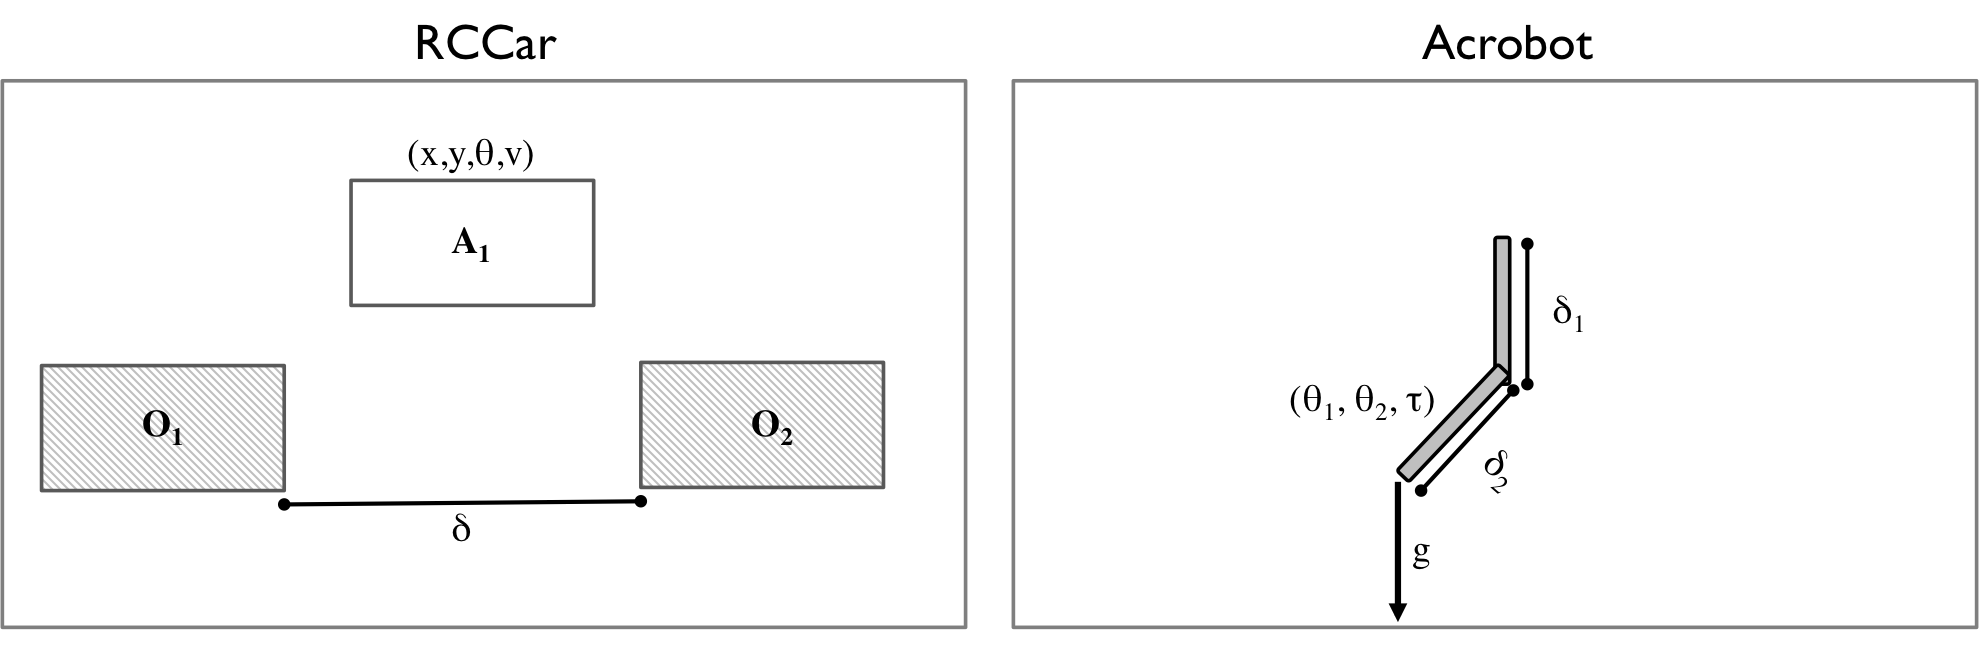
\includegraphics[width=\columnwidth]{swirl-experiments/domains.png}
 \caption{(A) Simulated control task with a car with noisy non-holonomic dynamics. The car ($A_1$) is controlled by accelerating and turning in discrete increments. The task is to park the car between two obstacles. \label{domains}}
\end{figure}

\subsubsection{Tasks}
For the car domain, the car can accelerate or decelerate in discrete $\pm 0.1$ meters per second squared increments (the car can reverse), and change its heading by $5^\circ$ degree increments.
The car's velocity and heading $\theta$ are inputs to a bicycle steering model which computes the next state.
The car observes its x position, y position, orientation, and speed in a global coordinate frame.
The car's dynamics are noisy and with probability 0.1 will randomly add or subtract $2.5^\circ$ degrees to the steering angle.
If the car parks between the obstacles, i.e., 0 speed within a $15^\circ$ tolerance and a positional tolerance of $1$ meter, the task is a success and the car receives a reward of $1$. 
The obstacles are 5 meters apart (2.5 car lengths).
If the car collides with one of the obstacles or does not park in 200 timesteps, the episode ends with a reward of $0$.

The acrobot domain consists of an under-actuated two-link pendulum with gravity and with torque controls on the joint. 
There are 4 discrete actions that correspond to clockwise and counter-clockwise torques on each of the links. 
The robot observes the angle $\theta_1, \theta_2$ and angular velocity $\omega_1, \omega_2$ at each of the links.
The dynamics are noisy where a small amount of random noise is added to each torque applied to the pendulum. 
The robot has 1000 timesteps to raise the arm above horizontal ($y=1$ in the image). If the task is successful and the robot receives a reward of $1$. 
The expected reward is equivalent to the probability that the current policy will successfully raise the arm above horizontal.


\subsubsection{Pure Exploration vs. \hirl}
In the first set of experiments, we compare the learning efficiency of pure exploration to \hirl (Figure \ref{exp:pe}).  The baseline line Q-Learning approach (QL) is very slow because it relies on random exploration to achieve the goal at least once  before  it  can  start  estimating  the  value  of  states  and actions. We fix the number of initial demonstrations provided to \hirl. We apply the segmentation and reward learning algorithms and construct a proxy task. In both domains, \hirl significantly accelerates learning and converges to a successful policy with significantly fewer demonstrations. We find that in the parallel parking domain this improvement is more substantial. This is likely because the task more naturally partitions into discrete subtasks. In the appendix, we visualize the segments discovered by the algorithm.

\begin{figure}[ht!]
\centering
 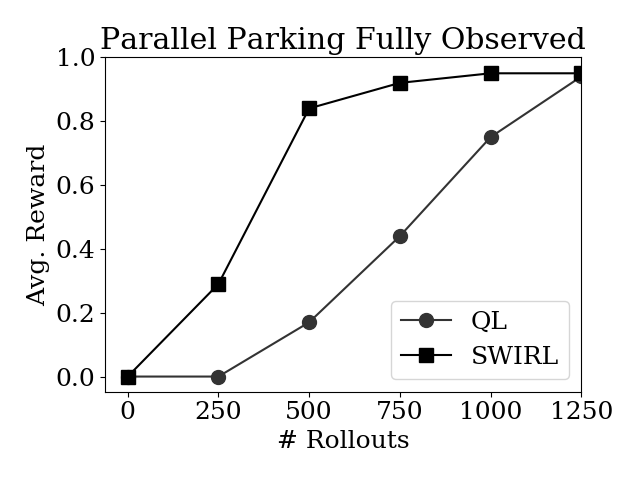
\includegraphics[width=0.48\columnwidth]{swirl-experiments/ppfo-rl1.png}
 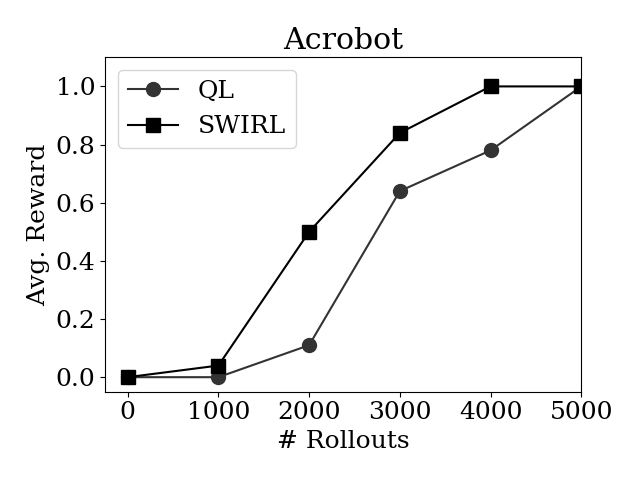
\includegraphics[width=0.48\columnwidth]{swirl-experiments/ppfo-rl2.png}
 \caption{Learning curves for Q Learning (QL) and \hirl on both simulated tasks. (Parallel Parking) For a fixed number of demonstrations 5, we vary the number of rollouts and measure the average reward at each rollout. (Acrobot) For a fixed number of demonstrations 15, we vary the number of rollouts and measure the average reward at each rollout. \label{exp:pe}}
\end{figure}


\subsubsection{Pure Demonstration vs. \hirl}
Next, we evaluate \hirl against a behavioral cloning approach  (Figure \ref{exp:pd}). We collect the initial set of demonstrations and directly learn a policy with an SVM. For the parallel parking task, we use a linear SVM. For the acrobot task, we use a kernel SVM with an RBF kernel. We fix the number of autonomous rollouts that \hirl can observe (500 for the parallel parking task and 3000 for the acrobot task). Note that the SVM technique requires observing the actions in the demonstration trajectories, which may not be possible in all applications. The SVM approach does have the advantage that it doesn't require any further exploration.
However, SWIRL and the pure demonstration approach are not mutually exclusive. 
As we show in our physical experiments, we can initialize Q-learning with a behavioral cloning policy. 
The combination of the two approaches allows us to take advantage of a small number of demonstrations and learn to refine the initial policy through exploration.


The SVM approach requires more than 10x the demonstrations to be competitive.
In particular, there is an issue with exhaustively demonstrating all the scenarios a robot may encounter. 
Learning from autonomous trials in addition to the initial demonstrations can augment the data without the burdening the supervisor.
Perhaps surprisingly, the initial dataset of demonstrations can be quite small.
On both tasks, with only five demonstrations, \hirl is within 20\% of its maximum reward. Representing a policy is often more complex than a reward function that guides the agent to valuable states. 
Learning this structure requires less data than learning a full policy.
This suggest that \hirl can exploit a very small number of expert demonstrations to dramatically reduce the number of rollouts needed to learn a successful policy.

\begin{figure}[ht!]
\centering
 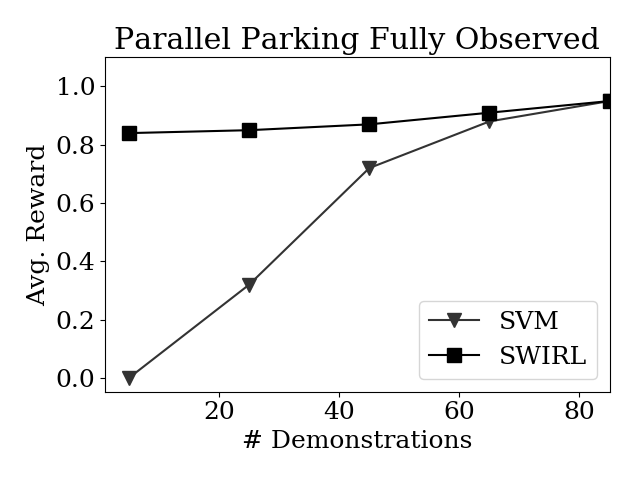
\includegraphics[width=0.48\columnwidth]{swirl-experiments/ppfo-svm1.png}
 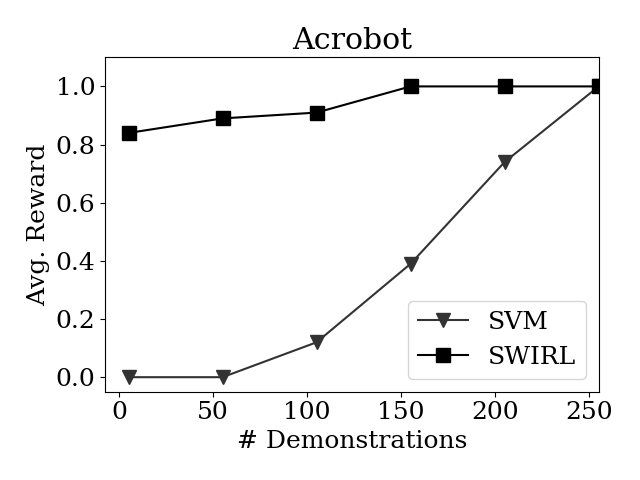
\includegraphics[width=0.48\columnwidth]{swirl-experiments/ppfo-svm2.png}
 \caption{Demonstration curves for imitation learning (SVM) and \hirl on both simulated tasks. (Parallel Parking) We fix the number of rollouts to $500$ and vary the number of demonstration trajectories each approach observes. (Acrobot) For a number of rollouts $3000$, we vary the number of demonstration trajectories given to each technique. \label{exp:pd}}
\end{figure}

\subsubsection{\hirl vs. Other Hybrid Approaches}
Finally, we compare \hirl to two other hybrid demonstration-exploration approaches (Figure \ref{exp:hyb}). The goal of these experiment is to show that the sequential structure learned in \hirl is a strong prior. As in the previous experiment, it is important to note that \hirl only requires a state-trajectory as a demonstration and does not need to explicitly observe the actions taken by the expert demonstrator.

Initializing the Q-Function with the demonstrations, did not yield a significant improvement over random initialization. This is because in expert demonstration one rarely observes failures, and if the q-learning algorithm does not observe poor decisions it will not be able to avoid them in the future. We also applied an IRL approach using estimated dynamics. The IRL approach is substantially better than the basic Q-Learning algorithm in the parallel parking domain. This is likely because it smooths out the sparse reward to fit a quadratic function. This does serve to guide the robot to the goal states to some extent. Finally, \hirl is the most sample-efficient algorithm. This is because the sequential quadratic rewards learned better align with the true value functions in both tasks. This structure can be learned from a small number of demonstrations.

\begin{figure}[ht!]
\centering
 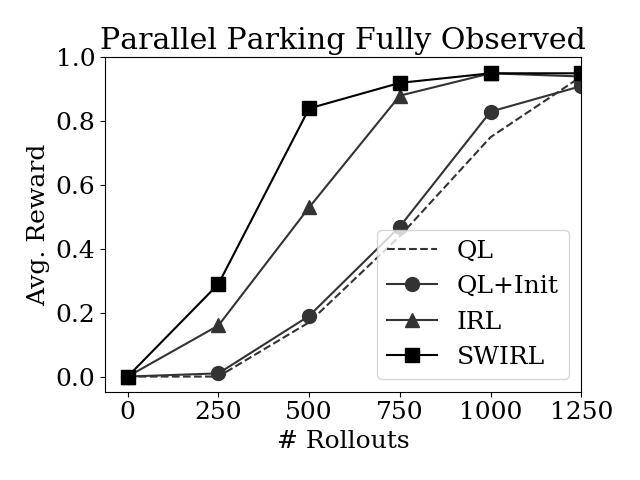
\includegraphics[width=0.48\columnwidth]{swirl-experiments/ppfo-irl1.png}
 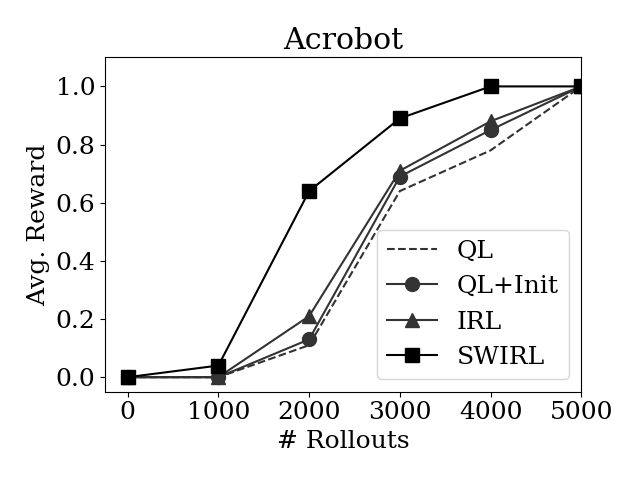
\includegraphics[width=0.48\columnwidth]{swirl-experiments/ppfo-irl2.png}
 \caption{Comparison of hybrid approaches. (Parallel Parking) For a fixed number of demonstrations 5, we vary the number of rollouts and measure the average reward at each rollout.  (Acrobot) For a fixed number of demonstrations 15, we vary the number of rollouts and measure the average reward at each rollout. \label{exp:hyb}}
\end{figure}

\begin{figure}[t]
\centering
 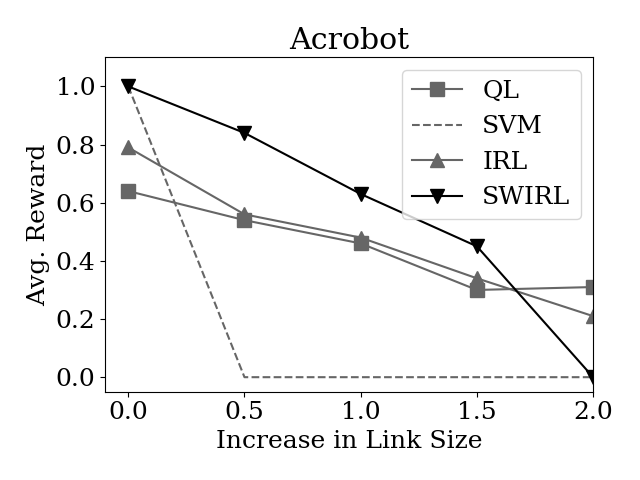
\includegraphics[width=0.8\columnwidth]{swirl-experiments/acr3.png}
 \caption{For a number of rollouts $3000$ and $250$ demonstrations, we measure the transfer as a function of varying the link size. (QL) denotes Q-learning, (SVM) denotes a baseline of behavioral cloning with a Kernel SVM policy representation, (IRL) denotes MaxEnt-IRL using estimated dynamics learned from the demonstrations, (SWIRL) denotes SWIRL. The SVM policy fails as soon the link size is changed. SWIRL is robust until the change becomes very large.  \label{exp:acr3}}
\end{figure}


\subsubsection{The Benefit Of Models}
Next, we consider the benefits of using Inverse Reinforcement Learning with the ground truth dynamics models compared to the ones estimated from data (Figure \ref{exp:mod}). One scenario where this problem setting is useful is when the demonstration dynamics (are known) but differ from the execution dynamics. Most common IRL frameworks, like Maximum Entropy IRL, assume access to the dynamics model. In the previous experiments, these models were estimated from data, and here we show the benefit of providing the true models to the algorithms. Both IRL and \hirl improve their sample efficiency significantly when ground truth models are given. This experiment illustrates that the principles behind \hirl are compatible with model-based methodologies.


\begin{figure}[ht!]
\centering
 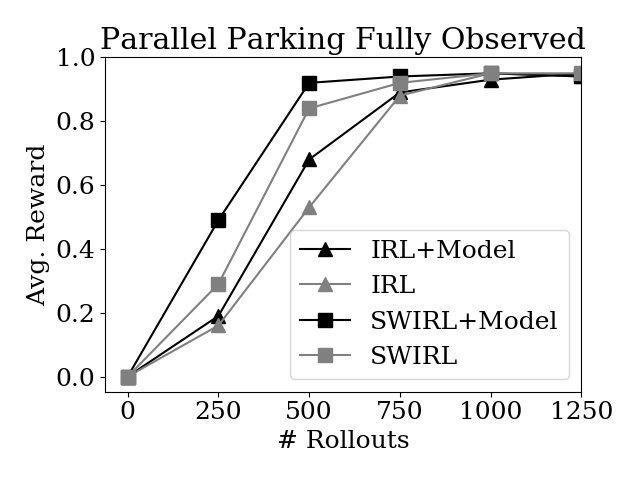
\includegraphics[width=0.48\columnwidth]{swirl-experiments/ppfo-mod1.png}
 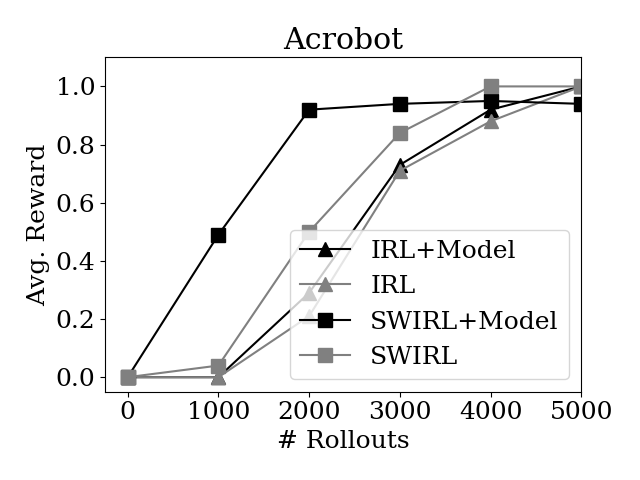
\includegraphics[width=0.48\columnwidth]{swirl-experiments/ppfo-mod2.png}
 \caption{(Parallel Parking) For a fixed number of demonstrations 5, we vary the number of rollouts and measure the average reward at each rollout.  (Acrobot) For a fixed number of demonstrations 15, we vary the number of rollouts and measure the average reward at each rollout. \label{exp:mod}}
\end{figure}


\subsubsection{Different Segmentation Methods}
In our general framework, \hirl is compatible with any heuristic to segment the initial demonstration trajectories. This heuristic serves to oversegment and the unsupervised learning model builds a model for sequential rewards from this heuristic. The previous experiments use a GMM-based approach as a segmentation heuristic, this experiment evaluates the same domains with other heuristics. In particular, we consider two other models: segmentation based on changes in direction of velocity and segmentation based on linear dynamical regimes. Figure \ref{exp:seg} illustrates the results. While there are differences between the performance of different heuristics, we found that the GMM-based approach was the most reliable across domains.

\begin{figure}[ht!]
\centering
 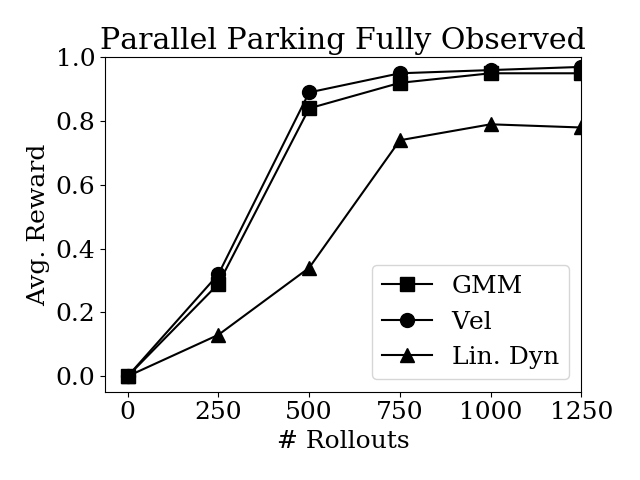
\includegraphics[width=0.48\columnwidth]{swirl-experiments/ppfo-seg1.png}
 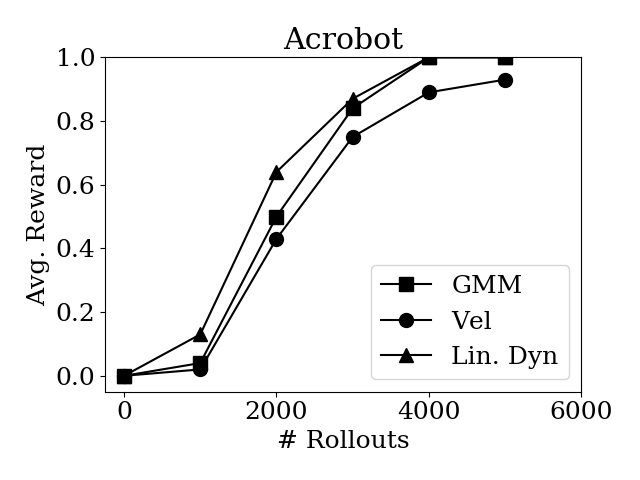
\includegraphics[width=0.48\columnwidth]{swirl-experiments/ppfo-seg2.png}
 \caption{We compare to different transition indicator heuristics with \hirl.  (Parallel Parking) For a fixed number of demonstrations 5, we vary the number of rollouts and measure the average reward at each rollout.  (Acrobot) For a fixed number of demonstrations 15, we vary the number of rollouts and measure the average reward at each rollout. \label{exp:seg}}
\end{figure}



\subsubsection{Transfer}
We constructed two transfer scenarios to evaluate situations whether the structure learned overfits to the initial demonstrations. In essense, this is an evaluation of how well the approaches handle transfer if the dynamics change between demonstration and execution.
We collect demonstrations $N=100$ on the original task, and then used the learned rewards or policies on a perturbed task.
For the parallel parking task, we modified the execution environment such that the dynamics are coupled in a way that turning right causes the car to accelerate forward by $0.05$ meters per second.
In the perturbed task, the car must learn to adjust to this acceleration during the reversing phase.
In the new domain, each approach is allowed $500$ rollouts. 
We report the results (Figure \ref{exp:pp-fo3}).

The success rate of the policy learned with Q-Learning is more or less constant between the two domains.
This is because Q-learning does not use any information from the original domain.
The SVM behavioral cloning policy has a drastic change.
On the original domain it achieves a 95\% success rate (with 100 demonstrations), however, on the perturbed domain, it is never successful.
This is because the SVM learned a policy that causes it to crash into one of the obstacles in the perturbed environment.

The IRL techniques are more robust during the transfer.
This is because the rewards learned are quadratic functions of the state and do not encode anything specific about the dynamics.
Similarly, in SWIRL, the rewards and transition regions are invariant to the dynamics in this transfer problem.
For SWIRL-E and SWIRL-G, there is only a drop of 5\% in the success rate.
On the other hand, the model-free version of SWIRL reports a larger drop of 16\%.
This is because the model-free version is not a true IRL algorithm and may enocde some aspects of the dynamics in the learned reward function.

Coincidentally, this experiment also shows us how to construct a failure mode for \hirl.
If the perturbation in the task is such that it ``invalidates'' a transition region, e.g., a new obstacle, then \hirl may not be able to learn to complete the task.
However, the transition regions give us a formalism to detecting such problems during learning as we can keep track of which regions are possible to reach.

\begin{figure}[ht!]
\centering
 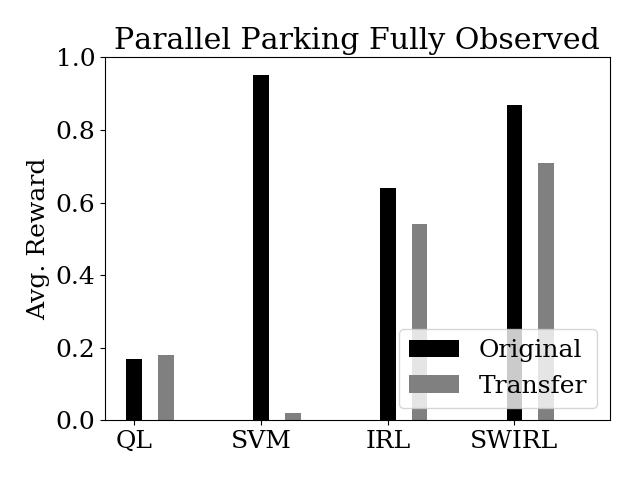
\includegraphics[width=0.8\columnwidth]{swirl-experiments/pp-fo3.png}
 \caption{For $500$ rollouts and $100$ demonstrations, we measure the robustness of the approaches to changes in the execution dynamics. (QL) denotes Q-learning, (SVM) denotes a baseline of behavioral cloning with a SVM policy representation, (IRL) denotes MaxEnt-IRL with estimated dynamics, and (SWIRL) denotes the model-free version of SWIRL. While the SVM is 95\% successful on the original domain, its success does not transfer to the perturbed setting. On the other hand, SWIRL learns rewards and segments that transfer to the new dynamics since they are state-space goals. \label{exp:pp-fo3}}
\end{figure}


As in the parallel parking scenario, we evaluate how the different approaches handle transfer if the dynamics change between demonstration and execution.
With $N=250$ demonstrations, we learn the rewards, policies, and segments on the standard pendulum, and then during learning, we vary the size of the second link in the pendulum.
We plot the success rate (after a fixed 3000 rollouts) as a function of the increasing link size (Figure \ref{exp:acr3}).

As the link size increases the even the baseline Q-learning becomes less successful. This is because the system becomes more unstable and it is harder to learn a policy.
The behavioral cloning SVM policy immediately fails as the link size is increased.
IRL is more robust but does not offer much of an advantage in this problem.
\hirl is robust until the change in the link size becomes large.
This is because for the larger link size, \hirl might require different segments (or one of the learned segments in unreachable).

\begin{figure}[ht!]
\centering
 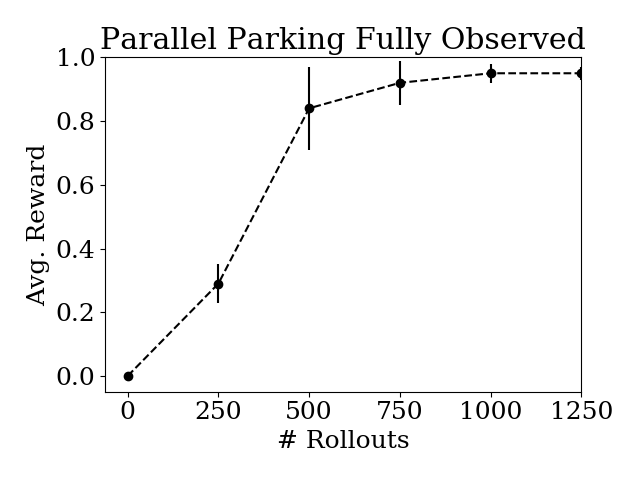
\includegraphics[width=0.48\columnwidth]{swirl-experiments/ppfo-eb1.png}
 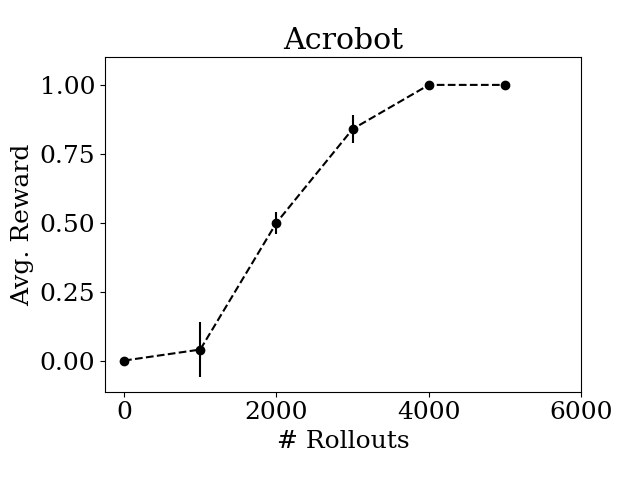
\includegraphics[width=0.48\columnwidth]{swirl-experiments/ppfo-eb2.png}
 \caption{Sensitivity of SWIRL. (Parallel Parking) We generate a random set of 5 demonstration, we vary the number of rollouts and measure the average reward at each rollout. We plot the mean and standard deviation over 100 trials.  (Acrobot) We generate a random set of 15 demonstration, we vary the number of rollouts and measure the average reward at each rollout. We plot the mean and 2 standard deviations over 100 trials \label{exp:eb}}
\end{figure}

\subsubsection{Sensitivity}
Next, we evaluated the sensitivity of \hirl to different initial demonstration sets (Figure \ref{exp:eb}). We sampled random initial demonstration sets and re-ran the algorithm on each of the two domains 100 times. Figure \ref{exp:eb} plots the mean reward as a function of the number of rollouts and 2 standard deviations over all of the trials. We find that \hirl is not very sensitive to the particular initial demonstration dataset. In fact, the 2 standard deviation error bar is less than the improvement in convergence in previous experiments.



\subsubsection{Segmentation and Partial Observation}
Next, we made the Parallel Parking domain more difficult to illustrate the connection between segmentation and memory in RL. 
We hid the velocity state from the robot, so the car only sees $(x,y,\theta)$. 
As before, if the car collides with one of the obstacle or does not park in 200 timesteps the episode ends.
We call this domain Parallel Parking with Partial Observation (PP-PO).

This form of partial observation creates an interesting challenge.
There is no longer a stationary policy that can achieve the reward.
During the reversing phase of parallel parking, the car does not know that it is currently reversing.
So there is ambiguity in that state whether to pull up or reverse.
We will see that segmentation can help disambiguate the action in this state.

As before, we generated 5 demonstrations using an RRT* motion planner (assuming deterministic dynamics) and applied each of the approaches.
The techniques that model this problem with a single MDP all fail to converge.
The Q-Learning approach achieves some non-zero rewards by chance.
The learned segments in \hirl help disambiguate dependence on history, since the segment indicator tells the car which stage of the task is currently active (pulling up or reversing)
After 250000 time-steps, the policy learned with model-based \hirl has a 95\% success rate in comparison to a <10\% success rate for the baseline RL, 0\% for MaxEnt-IRL, and 0\% for the SVM.


\begin{figure}[ht!]
\centering
 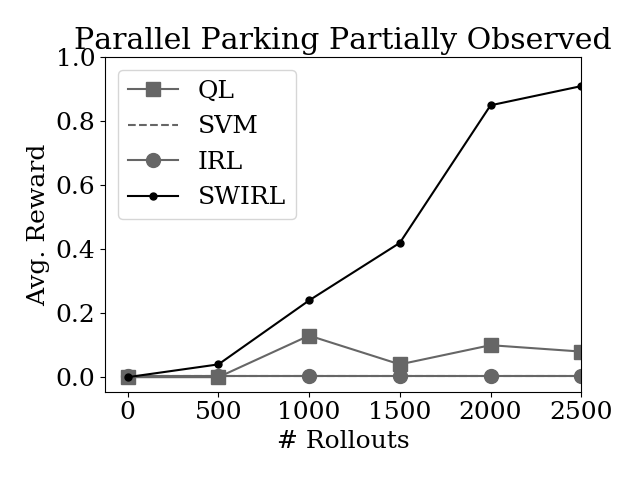
\includegraphics[width=0.8\columnwidth]{swirl-experiments/pp-po.png}
 \caption{We hid the velocity state from the robot, so the robot only sees $(x,y,\theta)$. For a fixed number of demonstrations $5$, we vary the number of rollouts and measure the average reward at each rollout. (QL) denotes Q-learning, (SVM) denotes a baseline of behavioral cloning with a SVM policy representation, (IRL) denotes MaxEnt-IRL with estimated dynamics, and (SWIRL) denotes SWIRL. SWIRL converges will the other approaches fail to reach a reliable success rate \label{exp:pp-po}}
\end{figure}



\subsection{Physical Experiments with the da Vinci Surgical Robot}
In the next set of experiments, we evaluate \hirl on two tasks on the da Vinci Surgical Robot.
The da Vinci Research Kit is a surgical robot originally designed for tele-operation, and we consider autonomous execution of surgical subtasks.
Based on a chessboard calibration, we found that the robot has an RMSE kinematic error of 3.5 mm, and thus, requires feedback from vision for accurate manipulation. 
In our robotic setup, there is an overhead endoscopic stereo camera that can be used to find visual features for learning, and it is located 650mm above the workspace.
This camera is registered to the workspace with a RSME calibration error of 2.2 mm.

\subsubsection{Deformable Sheet Tensioning} In the first experiment, we consider the task of deformable sheet tensioning. The experimental setup is pictured in Figure \ref{exp:dvrk3}. A sheet of surgical gauze is fixtured at the two far corners using a pair of clips. The unclipped part of the gauze is allowed to rest on soft silicone padding. The robot's task is to reach for the unclipped part, grasp it, lift the gauze, and tension the sheet to be as planar as possible.
An open-loop policy typically fails on this task because it requires some feedback of whether gauze is properly grasped, how the gauze has deformed after grasping, and visual feedback of whether the gauze is planar.
The task is sequential as some grasps pick up more or less of the material and the flattening procedure has to be accordingly modified.

The state-space is the 6 DoF end-effector position of the robot, the current load on the wrist of the robot, and a visual feature measuring the flatness of the gauze.
This is done by a set of fiducial markers on the gauze which are segmented by color using the stereo camera.
Then, we correspond the segmented contours and estimate a $z$ position for each marker (relative to the horizontal plane).
The variance in the $z$ position is a proxy for flatness and we include this as a feature for learning (we call this disparity).
The action space is discretized into an 8 dimensional vector ($\pm x$, $\pm y$, $\pm z$, open/close gripper) where the robot moves in 2mm increments.

We provided 15 demonstrations through a keyboard-based tele-operation interface.
The average length of the demonstrations was 48.4 actions (although we sampled observations at a higher frequency about 10 observations for every action).
From these 15 demonstrations, \hirl identifies four segments. Figure \ref{exp:dvrk3} illustrates the segmentation of a representative demonstration with important states plotted over time.
One of the segments corresponds to moving to the correct grasping position, one corresponds to making the grasp, one lifting the gauze up again, and one corresponds to straightening the gauze.
One of the interesting aspects of this task is that the segmentation requires multiple features.
Figure \ref{exp:dvrk3} plots three signals (current load, disparity, and z position), and segmenting any single signal may miss an important feature. 

Then, we tried to learn a policy from the rewards constructed by \hirl.
In this experiment, we initialized the policy learning phase of \hirl with the Behavioral Cloning policy.
We define a Q-Network with a single-layer Multi-Layer Perceptron with 32 hidden units and sigmoid activation.
For each of the segments, we apply Behavioral Cloning locally with the same architecture as the Q-network (with an additional softmax over the output layer) to get an initial policy. We rollout 100 trials with an $\epsilon=0.1$ greedy version of these segmented policies.

The learning results of this experiment are summarized below with different baselines.
The value of the policy is a measure of average disparity over the gauze accumulated over the task (if the gauze is flatter longer, then the value is greater).
As a baseline, we applied RL for 100 rollouts with no other information. RL did not successfully grasp the gauze even once.
Next, we applied behavioral cloning (BC) directly.
BC was able to reach the gauze and but not successfully grasping it.
Then, we applied the segmentation from \hirl  and applied BC directly to each local segment (without further refinement). 
This was able to complete the full task with a cumulative disparity score of $-3516$.
Finally, we applied all of \hirl and found the highest-value results ($-3110$).
For comparison, we applied \hirl without the BC initialization and found that it was only successful at the first two steps.
This indicates that in real tasks the initialization is crucial.

% Please add the following required packages to your document preamble:
% \usepackage[table,xcdraw]{xcolor}
% If you use beamer only pass "xcolor=table" option, i.e. \documentclass[xcolor=table]{beamer}
\begin{table}[ht!]
\centering
\scriptsize
\caption{Results from the deformable sheet tensioning experiment}
\label{my-label}
\begin{tabular}{llll}
\rowcolor[HTML]{000000} 
{\color[HTML]{FFFFFF} Technique} & {\color[HTML]{FFFFFF} \# Demonstrations} & {\color[HTML]{FFFFFF} \# Rollouts} & {\color[HTML]{FFFFFF} Value} \\
Pure Exploration (RL)                   & -                                        & 100                                & -8210                        \\
Pure Demonstration  (BC)                            & 15                                       & -                                  & -7591                        \\
Segmented Demos.                  & 15                                       & -                                  & -3516                        \\
\textbf{SWIRL}                  & 15                                       & 100                                & \textbf{-3110}                    
\end{tabular}
\end{table}


\subsubsection{Surgical Line Cutting}
In the next experiment, we evaluate generalization to different task instances.
We apply \hirl to learn to cut along a marked line in gauze similar to ~\cite{murali2015learning}.
This is a multi-step problem where the robot starts from a random initial state, has to move to a position that allows it to start the cut, and then cut along the marked line.
We provide the robot 5 kinesthetic demonstrations by positioning the end-effector and then following various marked straight lines.
The state-space of the robot included the end-effector position $(x,y)$ as well as a visual feature indicating its pixel distance to the marked line $(pix)$.
This visual feature is constructed using OpenCV thresholding for the black line.
Since the gauze is planar, the robot's actions are unit steps in the $\pm x, \pm y$ axes.
Figure\,\ref{exp:dvrk1} illustrates the training and test scenarios.

\hirl identifies two segments corresponding to the positioning step and the termination.
The learned reward function for the position step minimizes $x,y,pix$ distance to the starting point and for the cutting step the reward function is more heavily weighted to minimize the $pix$ distance.
We defined task success as positioning within $1$\,cm of the starting position of the line and during the following stage, missing the line by no more than $1$\,cm (estimated from pixel distance).
We evaluated the model-free version of \hirl, Q-Learning, and Behavioral Cloning with an SVM.
\hirl was the only technique able to achieve the combined task.

We evaluated the learned tracking policy to cut gauze.
We ran trials on different sequences of curves and straight lines. 
Out of the 15 trials, 11 were successful.
2 failed due to \hirl errors (tracking or position was imprecise) and 2 failed due to cutting errors (gauze deformed causing the task to fail).
1 of the failures was on the 4.5 cm curvature line and 3 were one the 3.5 cm curvature line.

% \begin{figure}[t]
% \centering
%  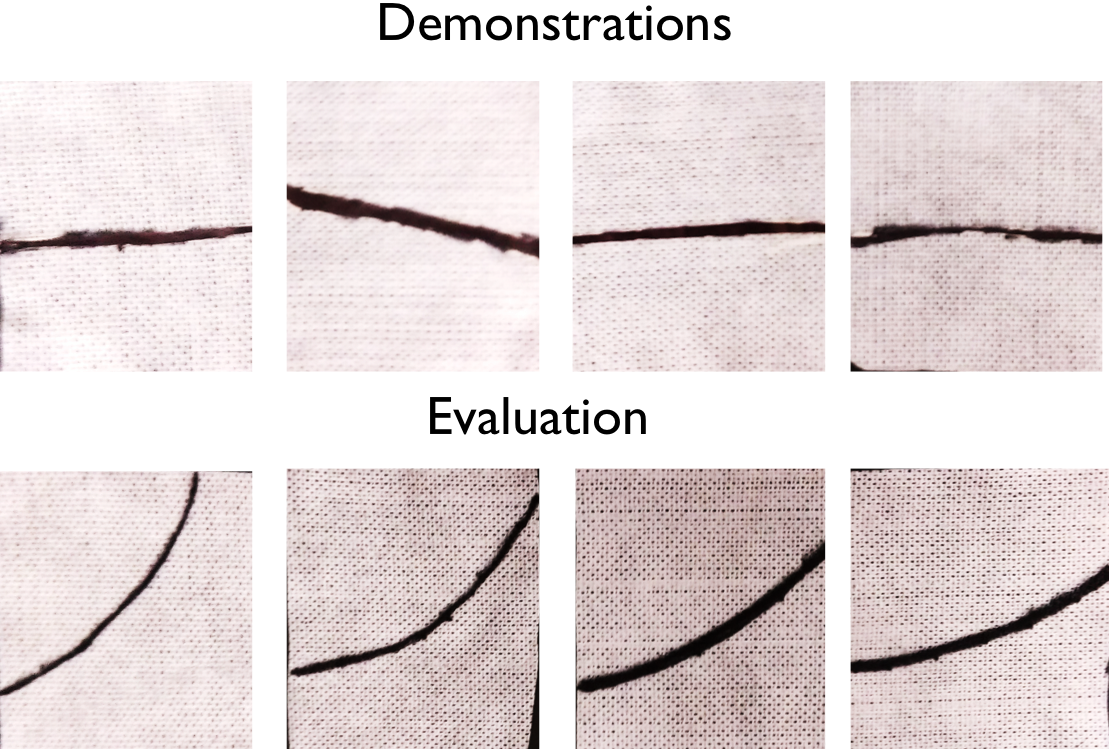
\includegraphics[width=0.7\textwidth]{swirl-experiments/dvrk-demos-1.png}
%  \caption{We collected demonstrations on the da Vinci surgical robot kinesthetically. The task was to cut a marked line on gauze. We demonstrated the location of the line without actually cutting it. The goal is to infer that the demonstrator's reward function has two steps: position at a start position before the line, and then following the line. We applied this same reward to lines that were not straight nor started in exactly the same position.\label{exp:dvrk1}}
% \end{figure}

% \begin{SCfigure}[10][t]
%     \centering
%     \vspace{-0.5em}
%     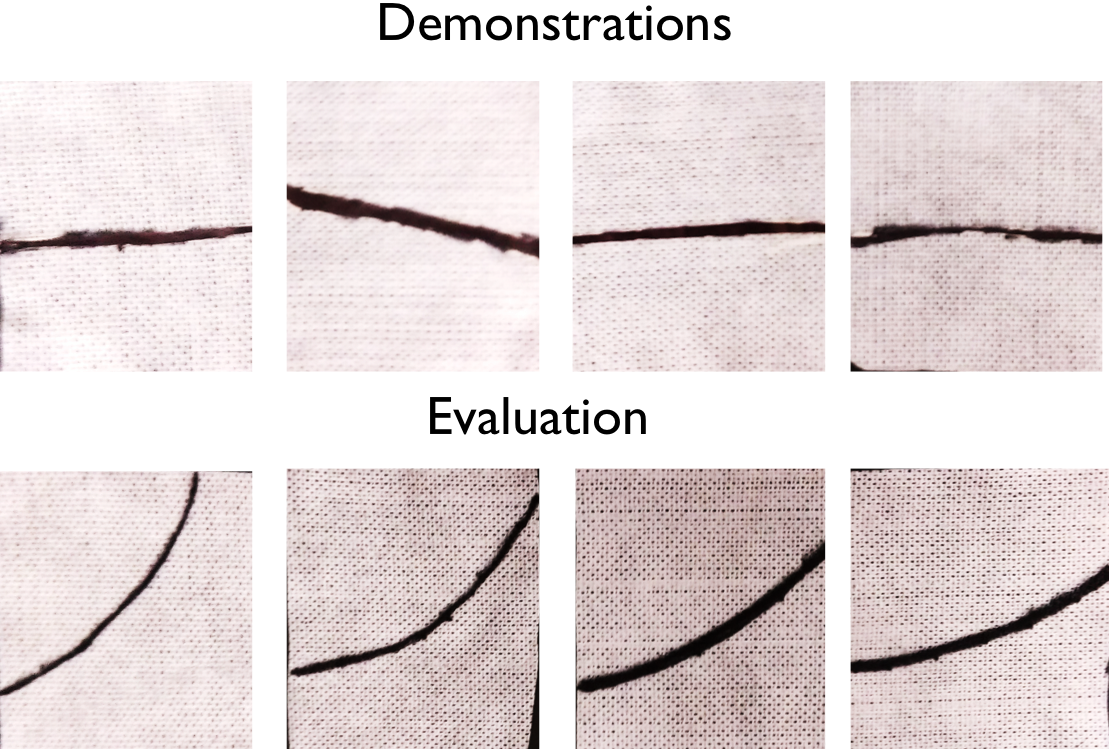
\includegraphics[width=0.5\textwidth]{swirl-experiments/dvrk-demos-1.png}
%     \caption{We collected demonstrations on the da Vinci surgical robot kinesthetically. The task was to cut a marked line on gauze. We demonstrated the location of the line without actually cutting it. The goal is to infer that the demonstrator's reward function has two steps: position at a start position before the line, and then following the line. We applied this same reward to lines that were not straight nor started in exactly the same position.}
%     \label{exp:dvrk1}
%     \vspace{-1.5em}
% \end{SCfigure}


\begin{figure}[ht!]
\centering
    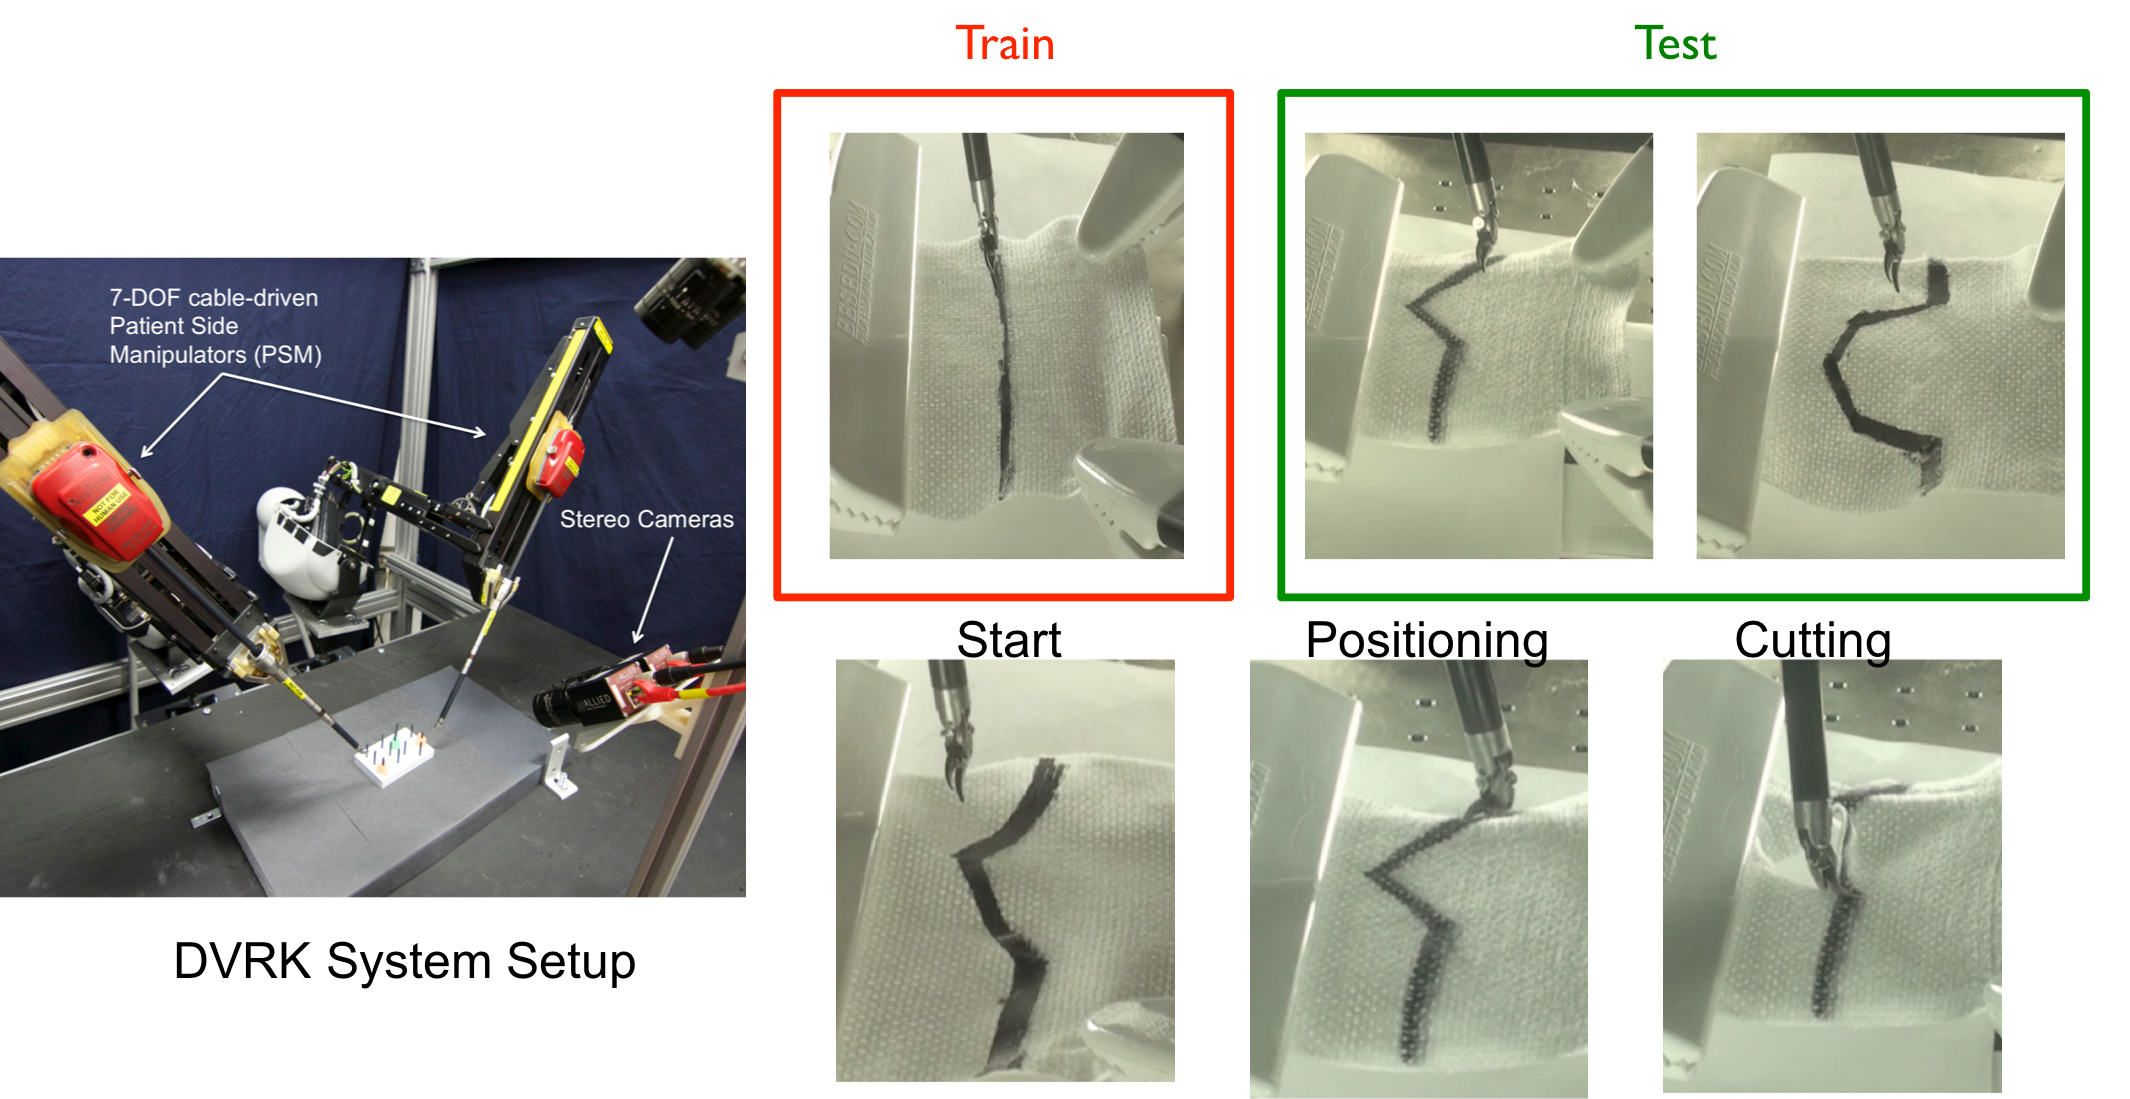
\includegraphics[width=\columnwidth]{swirl-experiments/dvrk-demo-2.png}
    \caption{
      We collected demonstrations on the da Vinci surgical robot kinesthetically. The task was to cut a marked line on gauze. We demonstrated the location of the line without actually cutting it. The goal is to infer that the demonstrator's reward function has two steps: position at a start position before the line, and then following the line. We applied this same reward to curved lines that started in different positions.
    }
    \label{exp:dvrk1}
% \vspace{-15pt}
\end{figure}

\begin{table*}[ht!]
    \centering
    \caption{With 5 kinesthetic demonstrations of following marked straight lines on gauze, we applied \hirl to learn to follow lines of various curvature. After 25 episodes of exploration, we evaluated the policies on the ability to position in the correct cutting location and track the line. We compare to SVM on each individual segment. SVM is comparably accurate on the straight line (training set) but does not generalize well to the curved lines.
    \label{dvrk:res1}}
    \resizebox{\linewidth}{!}{% put in textwidth
    \begin{tabular}{c||c|c|c|c}
    \hline
    \rowcolor[HTML]{CBCEFB} 
    Curvature Radius (cm) & SVM Pos. Error (cm) & SVM Tracking Error (cm) & \hirl Pos. Error (cm) & \hirl Tracking Error (cm) \\
     \hline \hline
    straight & 0.46 & 0.23 & 0.42 & 0.21  \\
    \rowcolor[HTML]{E0E0E0} 
    4.0 & 0.43 & 0.59 & 0.45 & 0.33 \\
    3.5 & 0.51 & 1.21 & 0.56 & 0.38 \\
    \rowcolor[HTML]{E0E0E0} 
    3.0 & 0.86 & 3.03 & 0.66 & 0.57 \\
    2.5 & 1.43 & {\color{red}-} & 0.74 & 0.87 \\
    \rowcolor[HTML]{E0E0E0} 
    2.0 & - & - & 0.87 & 1.45 \\
    1.5 & - & - & 1.12 & 2.44 \\
     \hline
    \end{tabular}
    }
    % \vspace{-10pt}
\end{table*}

Next, we characterized the repeatability of the learned policy.
We applied \hirl to lines of various curvature spanning from straight lines to a curvature radius of 1.5 cm.
Table \ref{dvrk:res1} summarizes the results on lines of various curvature.
While the SVM approach did not work on the combined task, we evaluated its accuracy on each individual step to illustrate the benefits of \hirl.
On following straight lines, SVM was comparable to \hirl in terms of accuracy.
However, as the lines become increasingly curved, \hirl generalizes more robustly than the SVM.
A single SVM has to learn both the positioning and cutting policies. The combined policy is much more complicated than the individual policies, e.g., go to a  goal and follow a line.





